% !TEX root = paper.tex
% !TEX encoding = UTF-8 Unicode

\section{Methodology}
\label{sec:methodology}

We hypothesize that the presentation of word-level alignment links to human post-editors may affect the quality or speed of the resulting output, and that such effects may be dependent on the quality of the underlying machine translations.
%
To test this hypothesis, we conduct a bilingual post-editing experiment where bilingual post-editors are presented with machine translation output of varying quality, with and without word-level alignment link visualization. 


% !TEX root = paper.tex
% !TEX encoding = UTF-8 Unicode


\begin{table}[t]
\begin{subtable}[b]{\linewidth}
\begin{center}
\caption{Russian-English adequacy evaluation guidelines}
\label{judge_guidelines_russian}
\begin{tabular} { | c | p{120mm} | }
\hline
  12 & The post-edited translation is superior to the reference translation \\ \hline
  10 & The meaning of the Russian sentence is fully conveyed in the English translation \\ \hline
  8 & Most of the meaning of the Russian sentence is conveyed in the English translation \\ \hline
  6 & The English translation misunderstands the Russian sentence in a major way, or has many small mistakes \\ \hline
  4 & Very little information from the Russian sentence is conveyed in the English translation \\ \hline
  2 & The English translation makes no sense at all \\ \hline
\end{tabular}
\end{center}
\end{subtable}
\ \\ \ \\
\begin{subtable}[b]{\linewidth}
\begin{center}
\caption{Spanish-English adequacy evaluation guidelines}
\label{judge_guidelines_spanish}
\begin{tabular} { | c | p{120mm} | }
\hline
  10 & The meaning of the Spanish sentence is fully conveyed in the English translation \\ \hline
%  9 & The English translation contains one minor error \\ \hline
  8 & Most of the meaning of the Spanish sentence is conveyed in the English translation \\ \hline
  6 & The English translation misunderstands the Spanish sentence in a major way, or has many small mistakes \\ \hline
  4 & Very little information from the Spanish sentence is conveyed in the English translation \\ \hline
  2 & The English translation makes no sense at all \\ \hline
\end{tabular}
\end{center}
\end{subtable}
\caption{Adequacy evaluation guidelines for bilingual Russian-English human judges \citep{2014_WMT_Schwartz_etal}, and for bilingual Spanish-English human judges \citep{2009_EACL_Albrecht_etal}. Because no reference translation was available for Spanish-English, the 12 category is omitted.}
\label{judge_guidelines}
\end{table}



\subsection{Bilingual Participants}

%All participants were bilingual graduate students enrolled in translations studies.

\subsubsection{Russian-English Bilingual Participants}
There were six participants who served as post-editors in the Russian-English portion of this study, all of whom were paid for their time.
%
These participants were all English-Russian bilinguals.
%
We designate these participants as PE1--PE6.
%
Four of the six bilingual participants (PE2, PE3, PE4, \& PE6) had Russian as their first language (L1) and were highly proficient in English as their second language (L2).
%
The other two bilingual participants (PE1 \& PE5) had English as their first language and were highly proficient in Russian as their second language.
%
Three of the six bilingual participants were graduate students and three were undergraduate students; all were enrolled in a university Russian Translation program. %and three were undergraduate students in the same program.
%a Russian Translation program at the same American university.

%In addition, we made use of monolingual post-editing data previously released by \citet{2014_WMT_Schwartz_etal}.
%
%The relevant participant in that study was a native English speaker with no knowledge of Russian.

\subsubsection{Spanish-English Bilingual Participants}

There were eleven participants who served as post-editors in the Spanish-English portion of this study, all of whom were paid for their time. 
%
They were all Spanish-English bilinguals.
%
We designate these participants as PE7--PE17. 
%
The first language (L1) of all eleven participants was English, and all eleven were highly proficient in Spanish as their second language (L2). 
%
These participants were students in a university Master of Spanish Translation program. 

\subsection{Source Language Data}

\subsubsection{Russian Data}

For the Russian-English portion of this study, we selected as source texts a subset of the texts from the 2014 Workshop on Statistical Machine Translation (WMT-14) shared translation task \citep{2014_WMT_Bojar_etal}.
%
Source texts were news articles covering world news events in late 2013.
%
The first text was originally a Russian-language BBC news article covering Syrian chemical weapons.
%
The second text was originally an English-language news article covering U.S. spying policy.
%
We designate the former as Doc A and the latter as Doc B.

These two texts were each divided into segments (32 and 33 segments, respectively) that corresponded to sentences or stand-alone phrases (typically corresponding to news headlines, captions, or cutlines).
%
Segments in Doc A varied in length from 3 to 35 words (mean length 17 words); 
%
segments in Doc B varied in length from 9 to 55 words (mean length 23 words).


Professional translations of Doc A into English and Doc B into Russian were commissioned as part of the WMT-14 shared translation task \citep{2014_WMT_Bojar_etal}.
%
%Doc A consists of 27 segments; Doc B has 28 segments.
%
The Russian version of each text was translated automatically using Moses \citep{2007_ACL_Koehn} by \citet{2014_WMT_Schwartz_etal} as part of their WMT14 shared task submission.
%
As a side effect of the phrase-based MT process, Moses can be configured to produce alignment links, indicating which target language words were produced from which source language words.
%
To enable maximal comparability with the post-editing results of \citet{2014_WMT_Schwartz_etal}, we make use of Russian-English machine translation results and alignments from that work here.



\subsubsection{Spanish Data}

Two Spanish source texts were selected. Both were extracts from a news article from a Spanish newspaper covering current world news events. 
%
The two texts were divided up into segments that corresponded to sentences or stand-alone phrases. 
%
The first text had 26 segments that varied in length from 4 to 24 words (mean length 15 words) and the second text had 25 segments that varied in length from 4 to 28 words (mean length 16 words).
%
We designate the former as Doc C and the latter as Doc D.
%
No reference translations exist for either Spanish text.

The Spanish source texts were translated automatically using Microsoft Bing Translator through its online developer API.
%
Bing Translator, when accessed via the developer API, can be configured to return character-level alignment links from source characters to target characters, in addition to translated target language sentences.
%
Our scripts derive word alignments from the character alignments returned by the Bing Translator API.



\subsection{Translation Quality}
\label{sec:translation_quality}

We hypothesize that any effects of word alignment visualization on post-editing may be dependent on the quality of the underlying machine translations displayed to the post-editors.
%
Because we care about the adequacy of post-edited translations, we consider actual human judgements to be preferable to automated metrics such as BLEU \citep{2002_ACL_Papineni_etal}, which at best serve as a flawed proxy for human judgements.
%
Instead, following \citet{2009_EACL_Albrecht_etal} and \citet{2014_WMT_Schwartz_etal}, we therefore obtained human judgements of translation adequacy for the Russian-English and Spanish-English machine translations used in this study.

The Russian language news articles used in this study have corresponding reference translations.
%
It is therefore possible (although given current machine translation quality, highly unlikely) that machine translation quality for any given segment could conceivably surpass the quality of the corresponding reference translation (if for example, the reference translator makes a mistake).
%
For assessing the quality of the Russian-English machine translations, then, we follow the 12-point adequacy scale of \citet{2014_WMT_Schwartz_etal}.
%
This adequacy scale is shown in Table \ref{judge_guidelines_russian} \vpageref[above]{judge_guidelines_russian};
%
this scale ranges from a low of 2 (the English translation makes no sense at all) to a high of 12 (the translation is superior to the reference).

The Spanish language news articles used in this study lack corresponding reference translations.
%
Thus, unlike the case of our Russian data, no matter how high the quality of machine translations, no Spanish-English machine translation segment could possibly receive a score of 12.
%
For Spanish-English, we therefore follow the 10-point adequacy scale of \citet{2009_EACL_Albrecht_etal}.
%
This adequacy scale is shown in Table \ref{judge_guidelines_spanish} \vpageref[above]{judge_guidelines_spanish};
%
this scale is very similar to the former, but has a high of 10 (the meaning of the source sentence is fully conveyed in the English translation) instead of 12.


% !TEX root = paper.tex
% !TEX encoding = UTF-8 Unicode


\begin{figure*}
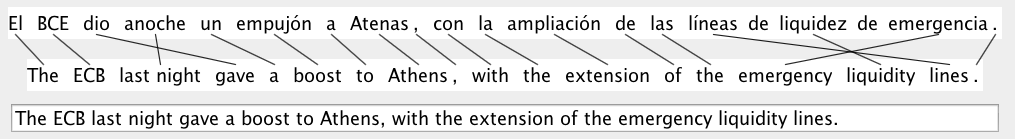
\includegraphics[width=\linewidth]{alignments_true}
\caption{Post-editing interface, with alignment links displayed. Sentence shown is from Spanish-English Doc C.}
\label{fig:screenshot_true}
\end{figure*}



\subsection{Post-Editing Interface}

For this study, we developed a novel post-editing interface, based on the open source software used and released by \citet{2014_WMT_Schwartz_etal}.
%
Our software is written using Scala \citep{2014_Scala_Odersky}, and is released as open source (see the software supplement that accompanies this work).
%
This code constitutes a ground-up rewrite of the Java-based post-editing interface of \citet{2014_WMT_Schwartz_etal}, written using a strict model-view-controller software design pattern to be easy for other researchers to use and extend.

Our post-editing interface can be seen in Figure~\ref{fig:screenshot_true} \vpageref[above]{fig:screenshot_true}.
%
Each text was presented to post-editors in one of two variant modalities --- word-level alignment links could either be visualized or left absent.
%
In both variants, each source language segment was presented along with the corresponding machine translated English segment; a text field (initially populated with the machine translated segment) where the post-editor could make changes was also presented.
%
In the first variant, the word-level alignment links produced by the machine translation decoder (Moses for Russian-English, Bing Translator for Spanish-English) were graphically displayed, linking source words to their corresponding machine translated target words.
%
In the second variant, the word-level alignment links were omitted from the visualization interface.


% !TEX root = paper.tex
% !TEX encoding = UTF-8 Unicode

\begin{figure}
\begin{subfigure}[b]{\linewidth}
\begin{center}
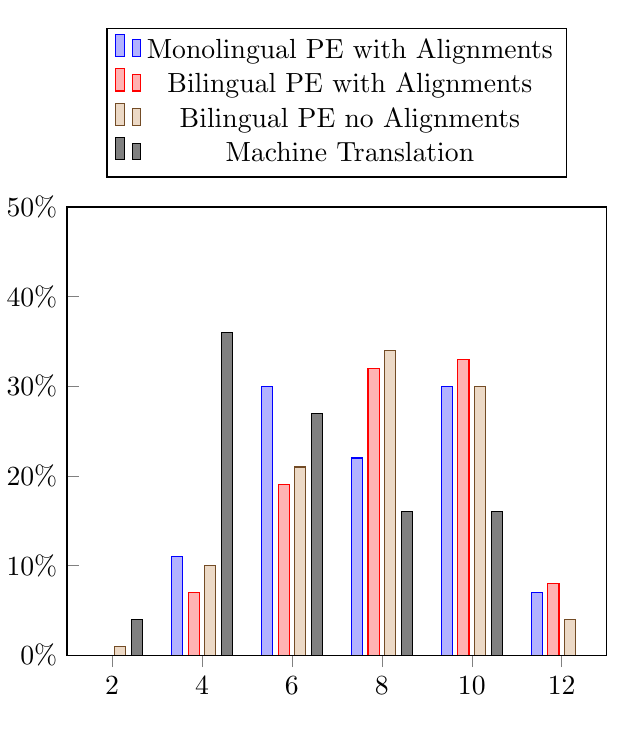
\begin{tikzpicture}[trim left={(-0.5,0)}]
\begin{axis}[
	%at={(10,0)},
	ymin=0,
	x tick label style={
		/pgf/number format/1000 sep=},
	ylabel shift={-0.15cm},
	ytick={0,10,20,30,40,50},
	yticklabels={0\%,10\%,20\%,30\%,40\%,50\%},
%	ymin={0},
	ymax={50},
%	ylabel={\%},
%	enlargelimits=0.15,
	xtick pos=left,
	ytick pos=left,
%	xlabel={XXXX YYY ZZZZ},
	%,
%	legend style={at={(0.5,-0.15)}},
%		anchor=north,legend columns=-1},
	legend style={at={(0.5,1.40)},anchor=north},
	ybar,
	bar width=4pt,
]
\addplot 
	coordinates {(4,11) (6,30) (8,22) (10,30) (12,7)};

\addplot 
	coordinates {(4,7) (6,19) (8,32) (10,33) (12,8)};

\addplot 
	coordinates {(2,1) (4,10) (6,21) (8,34) (10,30) (12,4)};

\addplot 
	coordinates {(2,4) (4,36) (6,27) (8,16) (10,16)};

\addplot[black,sharp plot,update limits=false] 
	coordinates {(-1,0) (14,0)};
	
\legend{Monolingual PE with Alignments,Bilingual PE with Alignments,Bilingual PE no Alignments, Machine Translation}
\end{axis}
\end{tikzpicture}
\end{center}
\caption{Russian-English}
\label{fig:percentage_segments_ru}
\end{subfigure}
\ \\
\begin{subfigure}[b]{\linewidth}
\begin{center}
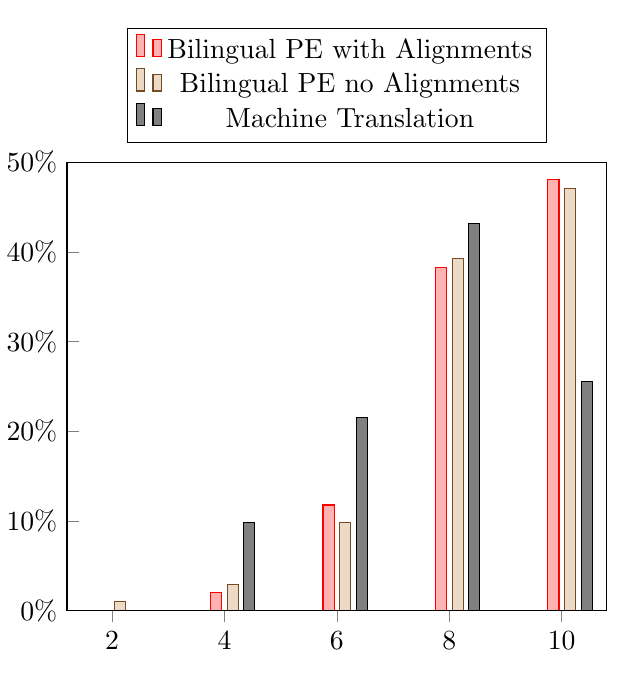
\begin{tikzpicture}[trim left={(-0.5,0)}]
\begin{axis}[
	%at={(10,0)},
	ymin=0,
	x tick label style={
		/pgf/number format/1000 sep=},
	ylabel shift={-0.15cm},
	ytick={0,10,20,30,40,50},
	yticklabels={0\%,10\%,20\%,30\%,40\%,50\%},
%	ymin={0},
	ymax={50},
%	ylabel={\%},
%	enlargelimits=0.15,
	xtick pos=left,
	ytick pos=left,
%	xlabel={XXXX YYY ZZZZ},
	%,
%	legend style={at={(0.5,-0.15)}},
%		anchor=north,legend columns=-1},
	legend style={at={(0.5,1.30)},anchor=north},
	ybar,
	bar width=4pt,
]
\addplot 
	coordinates {};

\addplot coordinates {(4,1.9607843137254901) (6,11.76470588235294) (8,38.23529411764706) (10,48.03921568627451) };
\addplot coordinates {(2,0.9803921568627451) (4,2.941176470588235) (6,9.803921568627452) (8,39.21568627450981) (10,47.05882352941176) };
\addplot coordinates {(4,9.803921568627452) (6,21.568627450980394) (8,43.13725490196079) (10,25.49019607843137) };

\addplot[black,sharp plot,update limits=false] 
	coordinates {(-1,0) (14,0)};
	
\legend{Bilingual PE with Alignments,Bilingual PE no Alignments, Machine Translation}
\end{axis}
\end{tikzpicture}
\end{center}
\caption{Spanish-English}
\label{fig:percentage_segments_es}
\end{subfigure}
\caption{Percentage of segments judged to be in each adequacy category. For each language pair, we report percentages for raw (unedited) machine translation output, as well as output post-edited by a bilingual post-editor with access to alignments and without access to alignments. For Russian-English, we additionally report percentages for output post-edited by a monolingual post-editor \citep{2014_WMT_Schwartz_etal} with access to alignments.}
\label{fig:percentage_segments}
\end{figure}

\subsection{Procedure}

Participants performed the test individually in an office setting and were instructed to minimally post-edit. 
%
Specifically, participants were asked to disregard issues of style and to focus on 
%
a) how well the translation conveyed the meaning of the source text, and 
%
b) the grammatical correctness of the translated segments. 
%
Participants sat in front of a computer that displayed the source texts divided up into segments (see Figure \ref{fig:screenshot_true} \vpageref[above]{fig:screenshot_true}). % (see \citet{2014_WMT_Schwartz_etal}).
%
Directly below each source text segment, its machine translation was displayed.
%
Below that was an active response area, where participants were asked to carry out the post-editing.

During initial data collection (the Russian-English condition), the only data collected was the final post-edited output and the overall time taken per text.
%
Subsequently, we enhanced the post-editing software with additional logging functionality, enabling the software to record key-logging and mouse-logging data.
%
For the subsequent Spanish-English condition, this enhanced software was utilized; for this condition millisecond-precision keyboard-event and mouse-event logs were recorded in addition to collecting final post-edited output and overall time taken per text.

We believe that scientific inquiry is at its strongest when experiments can be easily replicated, and when the raw and processed data from such experiments can be directly verified by reviewers, readers, and other experimenters.
%
In that spirit, all data and code produced or used in this work are provided in the attached dataset and software supplements.
%
This includes all logs, along with raw machine translation output, alignment data, post-edited output, adequacy judgements, post-editing software, and supplementary scripts.



\subsubsection{Russian-English Participant Assignment}




Each participant was instructed to edit one of the two texts using the interface where alignment links were shown,
%
and to edit the other text using the interface where alignment links were omitted.
%
Participants post-edited the two texts in one session lasting less than two hours, although there were no time limits set for the task.
%
Post-Editors 2, 4, and 6 were assigned to post-edit Doc A using the variant 1 interface that displayed alignments, and Doc B using the variant 2 interface that omitted alignments.
%
Post-Editors 1, 3, and 5 were assigned Doc A using variant 2 and Doc B using variant 1.

%For each of the segments there was also a reference translation created by XXXX.




\subsubsection{Spanish-English Participant Assignment}

Participants post-edited one text using the interface where alignment links were shown and the other text using the interface where alignment links were omitted. 
%
Participants post-edited the two texts in one session lasting less than one hour. 
%
Post-editors 7, 9, 11, 13, 15, and 17 edited Doc C using the interface that omitted the alignments and Doc D using the interface that displayed the alignments. 
%
Post-editors 8, 10, 12, 14, and 16 edited Doc C using the interface that displayed the alignments and Doc D using the interface that omitted the alignments.






